\documentclass[../../../main.tex]{subfiles}
 
\begin{document}
\label{sec:courseDesc}

\begin{table}
\centering
\begin{tabular}{| c | c | c | c | c |}
\hline \hline
Semester & Course & Credits & Students & Curriculum feature \\ \hline
Fall 2017 & PHYS135A-01 & 4.0 & 24 & Intro \\ \hline
Fall 2017 & PHYS150-01 & 4.0 & 17 & COM1/Intro \\ \hline
Spring 2018 & PHYS135B-01 & 4.0 & 18 & Intro \\ \hline
Spring 2018 & PHYS180-02 & 5.0 & 19 & COM1/Intro \\ \hline
Spring 2018 & COSC330/PHYS306 & 3.0 & 6 & Advanced \\ \hline
Fall 2018 & PHYS135A-01 & 4.0 & 24 & Intro \\ \hline
Fall 2018 & PHYS135A-02 & 4.0 & 26 & Intro \\ \hline
Jan 2019 & COSC390 & 3.0 & 8 & Advanced \\ \hline
Spring 2019 & PHYS135B-01 & 4.0 & 25 & Intro \\ \hline
Spring 2019 & PHYS180-02 & 4.0 & 9 & Intro/COM1 \\ \hline
Fall 2019 & PHYS135A-01 & 4.0 & 24 & Intro \\ \hline
Fall 2019 & PHYS150-02/03 & 4.0 & 26 & Intro/COM1 \\ \hline
Fall 2019 & INTD255 & 3.0 & 23 & CON2 \\ \hline
-- & Total & 50.0 & -- & -- \\ \hline
\hline
\end{tabular}
\caption{\label{tab:courses:teaching} This table is a summary of my courses since Fall 2017.  The introductory courses are 135A, 135B, 150, and 180.  The first advanced course PHYS306 is cross-listed as COSC330. The second advanced course, COSC390, is now listed as an official computer science course and counts towards the ICS major, as does COSC330.  I am currently teaching my first CON2 style course, INTD255 (see Sec. xx for details). Not included are my PHYS396 (physics research) courses.  This course helps to satisfy \textbf{departmental goals 2, 7, and 8.}}
\end{table}

\textbf{\textit{Algebra-based physics (135A/B)}}. Algebra-based physics, PHYS135A/B, is a two-semester integrated lecture/laboratory sequence covering Newton's Laws to electromagnetism\footnote{See supplemental material for example syllabi.}.  PHYS135 is a requirement for majors such as KNS and CHEM.  Students practice problem-solving with algebra, trigonometry, and vectors.  I employ a mixture of traditional and PER methods to satisfy \textbf{departmental goals 1, 4, and 6}.  The PER methods are \textit{Peer Instruction (PI)} and \textit{Physics Education Technology (PhET)}.  I no longer use JITT modules (see Sec. \ref{sec:oof}).  I have modified them in alignment with department and FPC recommendations.  My total teaching credits and number of students for this course is listed in Tab. \ref{tab:courses:teaching}.  \\ \hspace{0.1cm}

The first learning focus for non-majors is \textbf{curiosity}, with the measureable goals stated in Sec. \ref{sec:teaching_phil1}.  To satisfy the goal of increasing physics interest, students may present at the outset of class a recent science journal article pertaining to physics.  I incentivise the students to present with extra credit, and I help them to practice oral communication of scientific ideas (\textbf{Departmental goal 7})\footnote{Examples of such articles presented by students are included in the supplemental materials.}.  Once the students overcome nerves and try speaking in front of peers, I find that they begin to choose content that connects to their major.  It is fulfilling to see the students shine as they teach their peers.  \\ \hspace{0.1cm}

A second method I use to increase student curiosity is to require the students to design a physics experiment in small groups.  The OpenStax textbooks contain many workable examples they can build.  Each group must first submit a proposal in the middle of the semester.  I then help them refine it and ensure they have proper equipment.  After data collection, I invite them to office hours to coach them on the presentation\footnote{Included in the supplemental materials are examples of the students' final presentations.}.  Allowing the students to choose the topic and design is meant to give them an avenue for their curiosity.  Making this assignment an oral presentation also goes toward \textbf{Departmental goal 7}.  The data in Sec. \ref{sec:oof} show that the students \textit{are reporting an increase in their curiosity for physics}, and this trend is increasing over time. \\ \hspace{0.1cm}

The second introductory focus is \textbf{improvement of analysis skill}.  I use PI modules and PheT simulations as part of my strategy.  PI (Peer Instruction) modules were first developed by Eric Mazur \cite{mazur2013peer}, and have better performance than traditional content.  It is often helpful to illustrate physics concepts with PheT (Physics Education Technology) simulations, or to perform laboratory activities we cannot consruct (e.g. altering the strength of gravity)\cite{phet}.  These two modules are my main PER tools for boosting student problem-solving ability.  Following department and FPC recommendations, I have balanced the use of these two modules with the inclusion of more traditional content.  Finally, I have decided to cut JITT modules \cite{jitt} in favor of more example problems.  The students did not gain much from them, but express a desire for more step-by-step examples instead.  I have put this recommendation in place.  \\ \hspace{0.1cm}

\begin{figure}[ht]
\centering
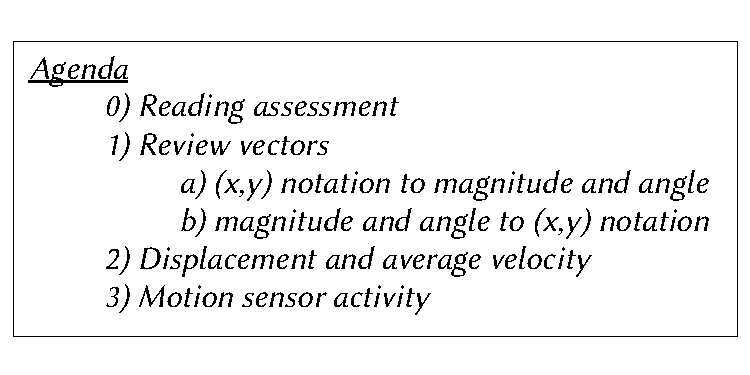
\includegraphics[width=0.45\textwidth]{ExampleAgenda.pdf}
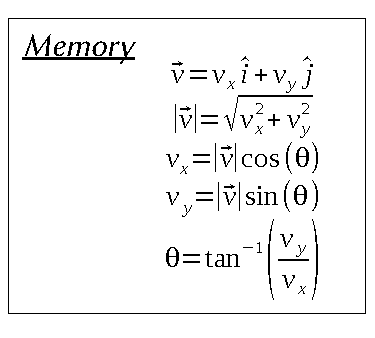
\includegraphics[width=0.22\textwidth]{ExampleMemory.pdf}
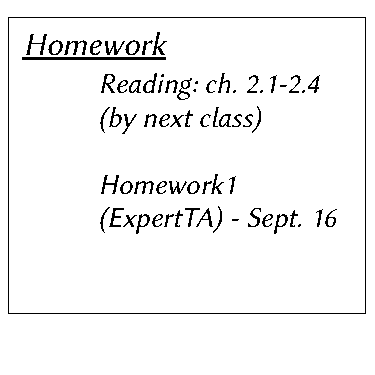
\includegraphics[width=0.22\textwidth]{ExampleHomework.pdf}
\caption{\label{fig:courses:intro:exampleAgenda} (Left) The class agenda presented on the white board is always concise and based on student progress.  It is presented to the students before each class period.  (Middle) The memory bank is a list of equations on the whiteboard used during class, and is a practice that I began using in 2017.  (Right) The homework box on the whiteboard now includes specific reading assignments, in addition to placing them on the syllabus.  This practice follows the suggestion of a student from a 2018 section of algebra-based physics (135A).}
\end{figure}

To structure class, I prepare my whiteboard in the pattern shown in Fig. \ref{fig:courses:intro:exampleAgenda}.  After explaining the agenda and homework, class begins with a reading assessment or the bonus article disussion mentioned above.  This is followed by warm-up examples from the memory bank (see Fig. \ref{fig:courses:intro:exampleAgenda}).  Next, I introduce new concepts on the projector screen, followed by several examples in traditional form on the whiteboard.  Third, I engage the students with a PI module pertaining to the concept just presented in traditional form.  PI modules begin with an exercise on the screen, with A-D multiple choice.  Our classrooms have a system that records student answers anonymously, and the students first answer individually.  I display the answer distribution (see Fig. \ref{fig:exampleData} below), and if fewer than 70\% of the class answers correctly I initiate \textbf{table discussions} (see Sec. \ref{sec:moduleType}).  \\ \hspace{0.1cm}

PER shows that students learn efficiently from peers explaining their reasoning.  Table discussions encourage this type of learning and  give me the chance to find the struggling students. Spending time with struggling students helps me build a relationship of trust, and relaxes their anxieties.  After short table discussions, students submit their answers again.  We observe the answer distribution shift toward the correct answer (see Fig. \ref{fig:exampleData}).  Further, if 70\% of students answer correctly initially, we move forward.  Thus, we accelerate the pace only if the students are ready.  This creates the possibility of a few students being left behind, so I have added the concept of WAT\footnote{e.g. ``What?'' A meme indicating confusion.}.  WAT corresponds to answer E, and it allows a lost student to notify me anonymously.  If I see one or more WATs, I provide another example.  \textit{This strategy ensures inclusivity in my introductory classes}, in that we strive to leave no one behind.  \\ \hspace{0.1cm}

The second-half of the lecture/laboratory format moves on to the laboratory activity or PheT module.  An example of the difference between traditional labs and PhET modules occurs in PHYS135B and PHYS180, which cover electromagnetism.  In these courses, we often build DC electric circuits.  If the circuit is constructable in our lab, we perform a traditional experiment in which we measure voltages and electric current to verify a principle such as Ohm's Law\footnote{Ohm's law states that the current observed is proportional to the voltage in the circuit.}.  If the circuit cannot be easily built in our lab, we simulate it virtually with PhET software.  Whenever possible, we first simulate the circuit in PhET, and then construct it to compare simulation and experiment.  The PI modules, PheT modules, and traditional lecture content complete my strategy for improving the students' analysis skill, and go towards \textbf{Departmental goals 1, 4, and 6}.  \textit{The student evaluation data in Sec. \ref{sec:oof} show great progress in the student evaluation questions pertaining to this learning focus.} \\ \hspace{0.1cm}

I employ several methods to reach my third introductory course learning focus, \textbf{applications to society}.  The obvious routes are the applications in the OpenStax texts \cite{openstax1} regarding kinesiology and medicine.  I develop special PI modules and example problems around topics such as motion/work/energy in the human body, nerve cells as DC circuit simulation, and lightning/weather.  Which modules I deploy depends on the semester.  After reflecting on recent semesters, I have noticed that learning what interests the students and including content specifically pertaining to their majors is highly beneficial to keep them engaged.  Dropping the JITT module also frees more class-preparation time to add material I know particular students will enjoy\footnote{See supplemental material for an example of such a unit.}. \\ \hspace{0.1cm}

Two final methods for my third learning focus are the article discussions and term-papers.  A nice example of the former occured during the past year when I had an environmental science major in PHYS135A/B who would find articles relating physics to climate change that used course concepts.  The whole class benefitted by learning how physics is used in the study of climate change.  Essentially, article presentations empower the students to choose topics they know to have an impact on our community.  Occasionally I give hints at articles which are of high-impact, and this prompt is all most timid students need to take the next step of preparing one for class.  For extra-credit, I offer term-papers asking students to explain the physics of a recent or past historical discovery.  Some brilliant examples have emerged, including the history of the first measurements of the distance between the Earth and the Sun\footnote{Included in the supplemental material.}.  The paper writing requires students to use course concepts to understand scientific breakthroughs, and it provides them a venue to practice writing about the societal impact of physics (\textbf{Departmental goal 7}).  \\ \hspace{0.1cm}

\textbf{\textit{Calculus-based physics (150/180)}}. Calculus-based physics, PHYS150/PHYS180, is a two-semester lecture/laboratory formatted sequence that covers calculus-based kinematics, mechanics, work/energy, and electromagnetism\footnote{See supplemental material for example syllabi.}.  My course format is essentially the same as 135A/B, where I employ a mixture of traditional and PER active learning methods to \textbf{satisfy departmental goals 1, 4, and 6}.  As in the algebra-based classes, I implement \textit{Peer Instruction (PI)} \cite{mazur2013peer} and \textit{Physics Education Technology (PhET)} \cite{phet} modules when necessary.  Because PHYS150 and PHYS180 require tools from calculus (MATH141 may be taken concurrently in the Fall semester), students new to calculus benefit from PhET simulations to help visualize calculus concepts.  Examples include operations with scalar and vector fields in electromagnetism, single-variable integrals and derivatives in kinematics, and line integral calculation of work and energy.  Some students understand these concepts through the mathematics, and others prefer to learn them graphically (an experience familiar to most math teachers).  My total teaching credits and number of students for this course is listed in Tab. \ref{tab:courses:teaching}. \\ \hspace{0.1cm}

My PHYS150/180 classes are taught with the same methods and format as the algebra-based courses, with the inclusion of the full calculus-based version of introductory physics concepts.  Since the subjects of calculus and Newton's Laws were developed concurrently, often by the same scientists, these two subjects are linked intrinsically.  During the warm-up phase of class, I will sometimes pose a calculus problem (when necessary) to familiarize the students with a technique that is required to understand the concepts we will encounter during class.  Occasionally (and this is especially true in PHYS180) the physics requires calculus concepts that the students have not encountered yet in their concurrent courses.  These cases usually involve vector calculus (Calculus III, or MATH241), which helps to explain electric and magnetic fields.  I gauge the comfort level of the students, and typically restrict my calculus content to traditional whiteboard content and examples.  \textit{As a rule, we do not place calculus concepts on exams that the students have not encountered in pre-requisite or concurrent courses}.  \\ \hspace{0.1cm}

In Sec. \ref{sec:oof}, I reflect on the student evaluation data in the same fashion as with the algebra-based courses.  Similar to the conclusions for PHYS135A/B, the data in Sec. \ref{sec:oof} show that calculus-based student date shows an increase in their curiosity for physics over time, and \textit{great progress in measures touching upon their problem solving skills.}  I received almost perfect scores for data collected from my most recent PHYS180 course.  Although the reduced class size made this easier to achieve, I have reflected on the fact that the students place a high value on \textit{building a relationship of trust with them} in order to satisfy their curiosity and increase their analysis abilities. \textbf{Include examples of final projects.} %Review their written responses.

\subsubsection{Descriptions of each Module Type}
\label{sec:moduleType}

The following descriptions provide more detail about our PER instructional modules, in list form.

\underline{PI Modules} - Implementation of an active learning strategy involving group problem solving and discussion.  Several good references are found in \cite{mazur2013peer} \cite{AAPTPI} \cite{PhysPort}.
\begin{itemize}
\item PI-based modules contain conceptual, multiple-choice questions for the class about a physical system.  The question corresponding to the results in Fig. \ref{fig:exampleData} was \\ \vspace{0.5cm} \textbf{``If the slope on a position vs. time graph is positive before a time $t_0$, zero at $t_0$, and negative after $t_0$, which of the following is true? \\ \vspace{0.5cm} A) The acceleration of the object was negative before and after $t_0$.  \\ B) The acceleration of the object was positive before $t_0$, then negative. \\ C) The acceleration of the object was positive before and after $t_0$. \\ D) The object had no acceleration.}
\item Students respond \textit{individually and anonymously} with an electronic device, and the distribution of answers for choices A-D is shown on the class screen (see Fig. \ref{fig:exampleData}).
\begin{figure}
\centering
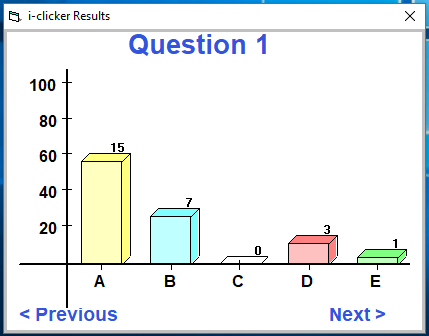
\includegraphics[width=0.45\textwidth,trim=0.25cm 1cm 0.15cm 2cm,clip=true]{FirstData.PNG}
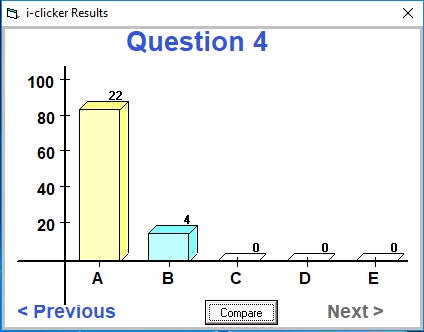
\includegraphics[width=0.45\textwidth,trim=0.25cm 1cm 0.15cm 2cm,clip=true]{SecondData.PNG}
\caption{\label{fig:exampleData} (Left) An answer distribution of my 25-student introductory algebra-based physics class, for a question that had a correct answer of A.  This distribution triggered a table discussion, because the fraction of correct answers was 0.6.  In addition, one student pressed E, indicating they were confused.  This prompts the professor to give a clue, or work another example.  (Right) After a table discussion with their peers, the students responded a second time, and the fraction of correct answers rose to 22/25 = 0.88.  The key concept for the question is that velocity and acceleration are not the same quantity (see text).}
\end{figure}
\item Students know to answer E if they are confused, and the anonymity is ensured so that students feel comfortable and the class is made more inclusive.
\item One of two actions is taken next:
\begin{enumerate}
\item If the fraction of correct answers to the conceptual question is larger than 0.7, class proceeds to the next exercise or new material.  This was the recommended fraction at the AAPT conference I attended in 2017.
\item If the fraction is less than 0.7, the professor initiates \textbf{table discussion}.
\end{enumerate}
\item \textbf{Table discussions} take place between students at the same table.  During this time the professor circulates, searching for the struggling students and answering questions.  After approximately 3-5 minutes, the discussion ends.
\item A second poll of the class is taken after table discussions, if they take place.  The \textit{shift} in the distribution towards the correct answer indicates an improved understanding of the concepts.  If the shift is not observed, the professor takes appropriate action.  If more than one person selects E, the material is covered again regardless of the shift.
\item The overall procedure is repeated for several exercises, and table discussions take place when necessary.  After several exercises, the class proceeds to new material, or the next concept in the unit.
\end{itemize}

\underline{PhET Modules} - Simulations written in HTML and JAVA, and published by The University of Colorado, Boulder, with public support from the National Science Foundation and private support from Google and the Moore and Hewlett Foundations \cite{phet}.  The goals of the simulations are that anyone should be able to operate them, and that they be based on proven PER.  The benefits of the simulations are researched and they are only published if the benefits to the students has been proven.
\begin{itemize}
\item The OpenStax textbooks for PHYS135 A/B and PHYS150/PHYS180 have built-in links to PhET simulations that allow students to illustrate concepts by visually simulating physics systems.
\item Several HTML5-based examples are here:
\begin{enumerate}
\item Electric charge and electric field: \url{https://phet.colorado.edu/en/simulation/charges-and-fields}
\item DC circuit construction: \url{https://phet.colorado.edu/en/simulation/circuit-construction-kit-dc}
\end{enumerate}
\item PhET simulations are incorporated into active learning in the classroom in four situations:
\begin{enumerate}
\item When a PhET simulation re-creates a laboratory measurement we are about to perform, it is useful to first simulate the expected results with the HTML or Java code and then perform the measurement to confirm the behavior of the system.
\item PhET simulations are also used when a desired measurement or experiment cannot be performed or constructed in the lab, such as altering gravity or changing the amount of friction between two surfaces.  Students benefit by being able to ``fine-tune'' a system, in order to expose the behavior of a system in real time.
\item PhET simulations are used to \textit{visualize} physical objects which are invisible.  Obvious examples are magnetic, electric, and gravitational fields, which are real but not (always) visible.
\item In special units, such as studying the behavior of electrical signals in the human body, there are PhET simulations from other fields (biology, chemistry, earth science, etc.) that prove useful to engage students' curiosity.
\end{enumerate}
\end{itemize}

\end{document}

